\section{Basic principals}

A digital filter is characterised as a \textit{linear time invariant} system referred to as a LTI system, which are to be described completely in the time domain by its impulse response $h[n]$. \\
When a discrete sequence $x[n]$ is applied to a LTI system it is the impulse response of the system $h[n]$ that determined what the output $y[n]$ will be. In other words the impulse response determine how much of the input sequence that passes the filter. \\ 
The output is determined by the convolution sum of input signal and impulse response of the system.
\begin{align}
y[n] = x[n]*h[n] = \sum_{k=1}^{\infty} x[k]h[n-k]
\end{align}  
The filters concerned in the project are referred to as frequency selective filters. ... that is why we what to go to the frequency domain.? \\
\\   
The frequency response of a filter is given by the Fourier transform of the impulse response, considering the input sequence $x[n]=e^{j\omega n}$ for $-\infty < n <\infty$, the frequency response is defined as\trine{side (40) DTSP}
\begin{align}
H(e^{j\omega})=\sum_{k=-\infty}^{\infty}h[k]e^{-j\omega k}
\end{align}
hence the outcome of the filter becomes 
\begin{align}
y[n]=H(e^{j\omega})e^{-j\omega n} \label{eq:filter_output}
\end{align} 
By \eqref{eq:filter_output} it is seen that $H(e^{j\omega})$ describes the change in complex amplitude of a complex exponential input signal to a given frequency. $H(e^{j\omega})$ is in general complex and hence it can be expressed as
\begin{align}
H(e^{j\omega})=|H(e^{j\omega})|e^{j\measuredangle H(e^{j\omega})}
\end{align}  
where $|H(e^{j\omega})|$ and $e^{j\measuredangle H(e^{j\omega})}$ are functions of \textit{magnitude} and magnitude of the filter respectively, both real valued and $2\pi$-periodic.\\ 
If the frequency response of a filter is real it is said to have \textit{zero phase}, which is equivalent to the phase response only tacking values that are integer multiples of $\pi$. Further if the frequency response can be written in the form 
\begin{align}
H(e^{j\omega})=A(e^{j\omega})e^{j(-\alpha\omega + j\beta)} 
\end{align}
where $\alpha$ and $\beta$ are constants and $A(e^{j\omega})$ is real,  the filter is said to have \textit{general linear phase}. That is because the phase response consist of constant terms added to the linear function making a straight line with slope $\alpha$ except from the discontinuities resolving from jumps of $2\pi$\trine{explain the discontinuity} \\
\\

When designing filters it is ideal to have approximately constant magnitude and zero phase corresponding to the frequency response. Though for causal systems\trine{define} zero phase is not possible to obtain, hence a linear phase response is acceptable and preferred over non linear phase.
\\
A measure of the linearity of the phase is the group delay. The group delay is...  \\    


\section{Ideal filter} 

\begin{figure}[H]
	\begin{subfigure}[b]{0.32\textwidth}
        \centering

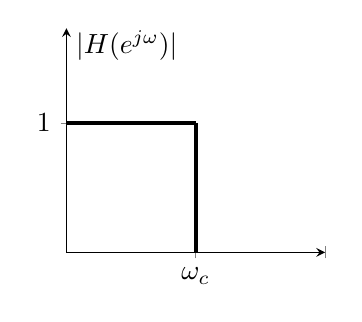
\begin{tikzpicture}[scale=1]
\begin{axis}[
scale=0.5,
unit vector ratio*=1 1 1,
axis lines = middle,
xtick={1.5,3},
xticklabels={$\omega_c$},
ytick={1.5},
yticklabels={$1$},
xmin=0,
xmax=3,
ymin=0,
ymax=2.6]
\node at (axis cs:0.7,2.4) {$|H(e^{j\omega})|$};
\draw[line width=0.5mm](axis cs:0,1.5)--(axis cs:1.5,1.5);
\draw[line width=0.5mm](axis cs:1.5,1.5)--(axis cs:1.5,0);
\end{axis}
\end{tikzpicture}
\caption{}
    \end{subfigure}
\begin{subfigure}[b]{0.32\textwidth}
        \centering

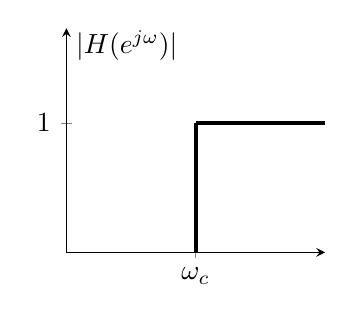
\begin{tikzpicture}[scale=1]
\begin{axis}[
scale=0.5,
unit vector ratio*=1 1 1,
axis lines = middle,
xtick={1.5},
xticklabels={$\omega_c$},
ytick={1.5},
yticklabels={$1$},
xmin=0,
xmax=3,
ymin=0,
ymax=2.6]
\node at (axis cs:0.7,2.4) {$|H(e^{j\omega})|$};
\draw[line width=0.5mm](axis cs:1.5,1.5)--(axis cs:3,1.5);
\draw[line width=0.5mm](axis cs:1.5,1.5)--(axis cs:1.5,0);
\end{axis}
\end{tikzpicture}

\caption{}
    \end{subfigure}
 \begin{subfigure}[b]{0.32\textwidth}
        \centering  
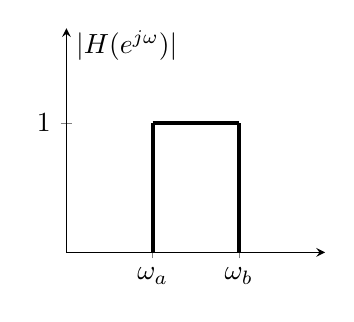
\begin{tikzpicture}[scale=1]
\begin{axis}[
scale=0.5,
unit vector ratio*=1 1 1,
axis lines = middle,
xtick={1,2},
xticklabels={$\omega_a$,$\omega_b$},
ytick={1.5},
yticklabels={$1$},
xmin=0,
xmax=3,
ymin=0,
ymax=2.6]
\node at (axis cs:0.7,2.4) {$|H(e^{j\omega})|$};
\draw[line width=0.5mm](axis cs:1,1.5)--(axis cs:1,0);
\draw[line width=0.5mm](axis cs:1,1.5)--(axis cs:2,1.5);
\draw[line width=0.5mm](axis cs:2,1.5)--(axis cs:2,0);
\end{axis}
\end{tikzpicture}

\caption{}
    \end{subfigure}

\caption{Magnitude of ideal (a) lowpass filter (b) highpass filter (c) bandpass filter}
\label{fig:ideal}
\end{figure}

\section{Filter design}

noter: \\
minimum phase system(side 250) when stable an casual system an invers system, if all zeros and pole are inside the unit circle 